\documentclass{standalone}
\usepackage{tikz}
\usetikzlibrary{arrows, positioning}

\begin{document}

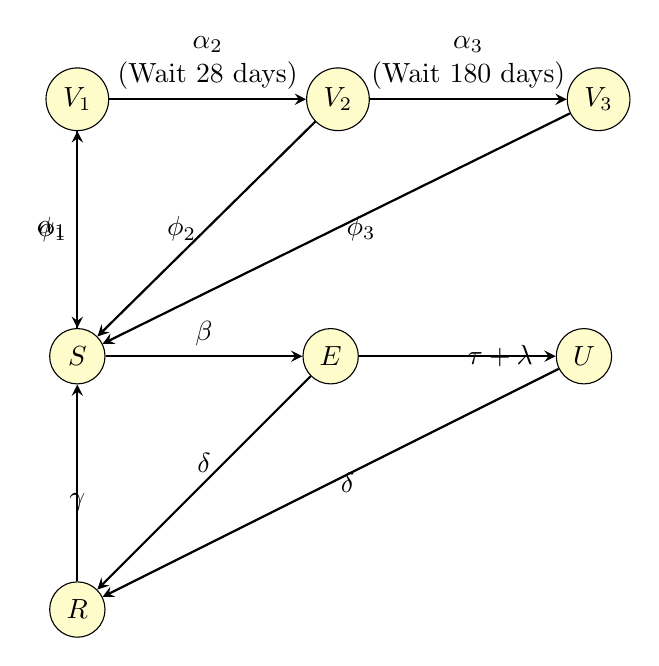
\begin{tikzpicture}[>=stealth, node distance=2.5cm, align=center]

    % Styles
    \tikzstyle{compartment} = [circle, draw, fill=yellow!20, minimum size=2em]
    \tikzstyle{arrow} = [->, thick]

    % Nodes
    \node[compartment] (S) {$S$};
    \node[compartment, right=of S] (E) {$E$};
    \node[compartment, right=of E] (U) {$U$};
    \node[compartment, below=of S] (R) {$R$};
    \node[compartment, above=of S] (V1) {$V_1$};
    \node[compartment, right=of V1] (V2) {$V_2$};
    \node[compartment, right=of V2] (V3) {$V_3$};

    % Arrows
    \draw[arrow] (S) -- node[above] {$\beta$} (E);
    \draw[arrow] (E) -- node[above] {$\delta$} (R);
    \draw[arrow] (E) -- node[right] {$\tau + \lambda$} (U);
    \draw[arrow] (U) -- node[right] {$\delta$} (R);
    \draw[arrow] (R) -- node[below] {$\gamma$} (S);

    \draw[arrow] (V1) -- node[left] {$\phi_1$} (S);
    \draw[arrow] (V2) -- node[left] {$\phi_2$} (S);
    \draw[arrow] (V3) -- node[right] {$\phi_3$} (S);

    \draw[arrow] (S) -- node[left] {$\alpha_1$} (V1);
    \draw[arrow] (V1) -- node[above] {$\alpha_2$ \\ (Wait 28 days)} (V2);
    \draw[arrow] (V2) -- node[above] {$\alpha_3$ \\ (Wait 180 days)} (V3);

\end{tikzpicture}

\end{document}